Tree algorithms can approximately calculate the forces in an 
$N$-body system by means of a hierarchical multipole expansion. 
This reduces the computational cost to something of order 
$O(N \ln N)$. On the download page of the lecture, a simple 
skeleton tree code can be downloaded (a C-version as well as a 
Python-version are provided). Note that this implementation uses 
only monopole order and is not optimized for speed or memory 
consumption. You can use this template for this exercise, 
either directly or translated to another language, or if you 
wish, you may also write your own tree code from scratch using 
the template as an example (it’s fun to do! ;-) ). \\
\\
Consider $N$ particles of total mass $M_{\textnormal{tot}}=1$ 
placed randomly into a cubical box of unit side length. For 
definiteness, we assume all particles have the same mass, and 
we adopt $G=1$. Assume that the gravitational potential of 
individual particles is Plummer-softened with a gravitational 
softening length $\varepsilon=0.001$, 
i.e. we adopt the potential
\begin{equation}
    \Phi(\vec r)=-\frac{m}{\sqrt{\vec r^2+\epsilon^2}}
\end{equation}
for a single particle of mass $m$.
Calculate the gravitational forces for all $N$ particles with an 
oct-tree and determine the typical force accuracy and 
calculational time in comparison with direct summation, both as 
a function of $N$ and of the opening angle parameter $\Theta^*$. 
To this end, carry out the following steps:


\paragraph{a) The idea of this exercise is that you use one of 
    the two templates provided (tree.c or tree.py \& call 
    tree.py). But if you like a challenge, you are encouraged 
    to write your own version! As a reference, there is pseudo 
    code provided at the end of the sheet.
} \ \\
    \\
    We chose to work with the template code (see below).


\newpage
\paragraph{b)
    The provided code template is incomplete, so start by filling 
    in the missing pieces. In particular, you need to add the 
    computation of the centers of mass and total masses of tree 
    nodes from their subnodes, as well as the partial force 
    calculation from a tree node that is used in the tree walk. 
    Also, please add a calculation of the exact forces by 
    direct summation. When you are done, verify that the force 
    approximation delivered by the tree code is roughly correct 
    by adding suitable output to the code.
} \ \\
    \\
    Computation of the centers of mass \& total masses of tree nodes: \\
    \\
    tree.py
    \lstinputlisting[firstline=98, lastline=123]{../code/ex8_tree/python/tree.py} \ \\
    \newpage \noindent
    Force calculation: \\
    \\
    tree.py
    \lstinputlisting[firstline=125, lastline=156]{../code/ex8_tree/python/tree.py} \ \\
    \\
    Calculation of exact forces: \\
    \\
    call\_tree.py
    \lstinputlisting[firstline=86, lastline=101]{../code/ex8_tree/python/call_tree.py}

\newpage
\paragraph{c)
    To allow a more quantitative analysis, add an automatic 
    measurement of the average force error after all forces 
    have been calculated by the tree and direct summation.
} \ \\ 
    \\
    To this end, consider the relative force error
    \begin{equation}
        \eta
        =\frac{\vec{a}_\textnormal{tree}-
        \vec{a}_\textnormal{direct}}{\vec{a}_\textnormal{direct}}
    \end{equation}
    for each particle, and determine a simple arithmetic average 
    $\langle\eta\rangle$ of the mean relative force error. Also, 
    add diagnostic code that tells you the average number of 
    particle-node interactions per particle, i.e. how many nodes 
    the multipole expansion on average involves. \ \\
    \\
    Our implementation can be seen below: \\
    \\
    call\_tree.py
    \lstinputlisting[firstline=103, lastline=108]{../code/ex8_tree/python/call_tree.py}


\newpage
\paragraph{d) Make a little grid of calculations for 
    $N=5000, 10000, 20000$ and $40000$, and opening angles 
    $\theta^*=0.2$, $0.4$ and $0.8$. In each case, measure the 
    calculation time for the tree-based force calculation and 
    for direction summation, as well as $\langle\eta\rangle$ 
    and the mean number of terms the tree code used per particle. 
    Report the results in a table.
} \ \\
    \\
    NOTE: For direct summation with $N=40000$ particles the 
    calculation could take very long; you can extrapolate from 
    smaller $N$ cases since we know it scales as $N^2$.
    Especially Python users might need to run smaller resolution 
    problems, e.g. divide the number by ten (however, you should 
    still have at least four different $N$ to be able to 
    extrapolate). \\
    \\
    We used Python, therefore we chose to test the algorithm on 
    $N=$ 2500, 5000, 10000 and 20000.
    \begin{table}[h!]
        \begin{center}
        \caption{$t_\textnormal{tree}$ (top) and $t_{N^2}$ (bottom) in seconds}
        \begin{tabular}{c | c | c | c}
            $N$ \textbackslash\ $\theta^*$ & 0.2  & 0.4  & 0.8 \\
            \hline
            2500  & 92   & 25   & 5    \\
                  & 50   & 47   & 47   \\
            \hline
            5000  & 234  & 55   & 11   \\
                  & 168  & 188  & 192  \\
            \hline
            10000 & 755  & 198  & 29   \\
                  & 1574 & 1455 & 1467 \\
            \hline
            20000 & 2666 & 598  & 214  \\
                  & 3888 & 4666 & 4915 \\
        \end{tabular}
        \end{center}
    \end{table} 
    \begin{table}[h!]
        \begin{center}
        \caption{mean number of interactions}
        \begin{tabular}{c | c | c | c}
            $N$ \textbackslash\ $\theta^*$ & 0.2  & 0.4  & 0.8 \\
            \hline
            2500  & 3444 & 824  & 180 \\
            \hline
            5000  & 4020 & 981  & 202 \\
            \hline
            10000 & 5141 & 1155 & 226 \\
            \hline
            20000 & 6220 & 1314 & 248 \\
        \end{tabular}
        \end{center}
    \end{table} 
    \begin{table}[h!]
        \begin{center}
            \caption{relative error $\langle\eta\rangle$}
            \begin{tabular}{c | c | c | c}
                $N$ \textbackslash\ $\theta^*$ & 0.2 & 0.4 & 0.8 \\
                \hline
                2500  & $(0.18\pm0.05)\%$ & $(0.96\pm0.12)\%$ & $(29.44\pm31.82)\%$ \\
                \hline
                5000  & $(0.13\pm0.02)\%$ & $(1.10\pm0.22)\%$ & $(8.18\pm1.96)\%$ \\
                \hline
                1000  & $(0.24\pm0.12)\%$ & $(1.05\pm0.20)\%$ & $(8.89\pm2.79)\%$ \\
                \hline
                20000 & $(0.26\pm0.14)\%$ & $(1.01\pm0.27)\%$ & $(8.66\pm5.71)\%$ \\
            \end{tabular}
        \end{center}
    \end{table} \ \\ 
    \red{hier noch was vergleichen/beschreiben?}

\newpage
\paragraph{e)
    Using the previous results, make a plot of the execution 
    time of the force calculation with the tree as a function of 
    $N$ (for the $\theta_c=0.4$ case). Use logarithmic axes and 
    fit a regression line (in the log) to the 4 data points you 
    obtained. Also include the results for direct summation. 
    Estimate the time needed for $10^{10}$ particles for both 
    methods.
} \ \\
    \begin{figure}[h!]
        \centering
        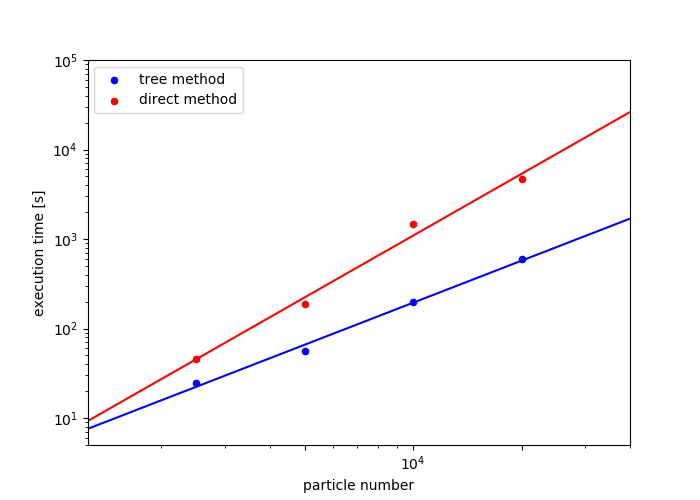
\includegraphics[width=\textwidth]{../plot/runtimes.png}
        \caption{execution time vs. particle number}
    \end{figure} \ \\ 
